\tightsection{Predictability of quality outcomes}
\label{predictability}

\jc{There is a serious problem of inconsistent use of quality sample and session. Need to clean up as soon as possible.}

The quality of a video session depends on a variety of factors,
including the network and the CDN. While many of these factors are not
under our control, some of them are. In our case, we assume that we
can control the bitrate of the session, as well as the CDN it streams
from. The challenge is that we do not know what quality will a session
exhibit given a particular choice of the parameters we can
control. This means that making any decision to change the CDN or the
bitrate is more or less like ``shooting in the dark''.

To address this problem, we start with the assumption that the session
quality is correlated to the different characteristics (attributes)
associated with the session. Example of such attributes are CDN,
bitrate, ISP, IP address, device, connectivity type, etc. We say that
a session is {\it predictable} if given the values of the attributes
associated with the session we can predict its quality. 

In this section, we formally define {\it predictability}, as well as
provide an upper bound to help us evaluate different prediction
algorithms (\Section~\ref{subsec:upperbound}). We then use our data
set to quantify this upper bound
(\Section~\ref{subsec:videoupperbound}).

%The quality outcome of a session which we would like to predict (which we will call the {\it session under prediction}) intuitively result from a diverse set of factors -- user behavior, network behavior, and CDN behavior, to name a few.  Many of these factors are out of our control; in other cases, a factor may be impacted in principle but its dependence on our decisions is unpredictable.  Our hope in approaching this problem is that some of them, and their causal dependence on decisions we can take, are consistently associated with characteristics we observe about sessions.  As shorthand we say that quality is {\it predictable} to extent that the impact of available decisions can be predicted, with low average error, using the available information about attributes of a session.  The first empirical question we must answer is whether quality is predictable in our dataset. 

%In this section, we first introduce the {\it predictability} and its upper bound of a set of sessions against a simple abstract model of prediction algorithm (\Section~\ref{subsec:upperbound}). Note that since the predictability is defined against a class of prediction algorithms that we consider rather than one specific design, its upper bound provides the insight of the intrinsic difficulty in predicting a set of sessions. We also quantify the predictability upper bound of video quality using our dataset (\Section~\ref{subsec:videoupperbound}). 


\tightsubsection{Definition and model}
\label{subsec:upperbound}

First, we define {\it prediction accuracy} of a set of sessions $s_1,\dots,s_n$ as follows. Given the a quality metric\footnote{In this section, we only consider one quality metric at a time.}, let $q(s_i)$ be the actual quality and $p(s_i)$ be the prediction on the quality. Then, the prediction accuracy $R((q_i,p_i)_{i=1,\dots,n})$ is defined as the correlation coefficient between $(q_1,\dots,q_n)$ and $(p_1,\dots,p_n)$~\cite{?}.

Then, we define attribute combination and attribute-based prediction algorithms.
An {\it attribute combination} ({\it AC}) $g$ is a tuple of attributes. Given an AC $g$, function $v_g$ takes a session $s$ as input and returns an array of values of $s$ on each attribute in $g$. For instance, if $g=[\textrm{ASN, CDN}]$, $v_g(s)=[ASN_s,CDN_s]$ where the client of $s$ belongs to $ASN_s$ and the server belongs to $CDN_s$.

An {\it attribute-based prediction algorithm} $P$ is defined by an AC $g$. $P$ takes a session $s$, and returns $P_g(s)$ as the prediction of quality outcome. 
The goal of prediction model is to identify the limitation of prediction accuracy when using only the information provided by these attributes. To generalize as much as possible, the only constraint of attribute-based prediction algorithm is that it has to give same prediction for all sessions under prediction if their values on every attributes in $g$ is identical. We call a set of sessions an {\it identical group} of $g$ if they have same value on all attributes in $g$. For instance, if $g=[\textrm{ASN, CDN}]$, then for two sessions $s_1,s_2$ in the identical group of $g$, i.e., $v_g(s_1)=v_g(s_2)$, the predicted quality of both of them must be the same, i.e., $P_g(s_1)=P_g(s_2)$. 


The predictability upper bound of a set of sessions is a measure of the capacity of a class of prediction algorithms, defined as the maximum prediction accuracy. The predictability upper bound of an AC on a set of sessions is defined as following. 
For an identical group of $g$, $s_1,\dots,s_n$, let their actual quality be $q_1,\dots,q_n$. Then, any attribute-based prediction algorithm of $g$ is going to give same prediction, $p$. The best prediction is $p^*=\textrm{argmax}_p R((q_i,p)_{i=1,\dots,n})$, so $p^*$ is the average value of $\bar{q_i}$. Now, the upper bound of prediction accuracy (which we will call {\it predictability upper bound}) of $g$ on an identical set of $g$, $s_1,\dots,s_n$, is $$R^*_g(s_{i,i=1,\dots,n})=R((q_i,p)_{i=1,\dots,n})$$. This definition can be easily extended to any set of sessions by dividing sessions into identical groups of $g$. 

The predictability upper bound quantifies the dispersion in quality of the sessions that an AC cannot differentiate. Ideally, if the attributes in AC $g$ selected reflect all the factors that determine the quality of a session, then the sessions in an identical group of $g$ should produce the same quality and the upper bound is exactly one. 

\tightsubsection{Predictability upper bound of video quality}

In this section, we quantify the predictability upper bound of the attributes in we observe on our dataset. 


There are two types of attributes to aggregate sessions. Given the same spatial attributes, temporal attributes (e.g., 1 minute) indicate the granularity in time which we use to differentiate sessions. Given the same temporal attributes, the spatial attributes (e.g., ASN, CDN) indicate the aspects of a session that we believe can make an impact on the quality.
We first quantify the impact of different spatial (e.g., full set or a subset) and temporal (1 hour or 10 second) attributes on predictability upper bound. Then we show that the predictability upper bound varies significantly among different partition of the dataset (e.g., Site).

\myparatight{Temporal attributes} 

\myparatight{Spatial attributes}

\myparatight{Predictability upper bound of different partitions}


\tightsubsection{Summary of observations}
\begin{packedenumerate}
	\item The overall prediction accuracy
\end{packedenumerate}


\tightsection{Challenges of A Practical Prediction Algorithm}

\comment{
We then investigate a naive prediction algorithm that make prediction by only looking at sessions sharing exact values on all attributes, and categorize its reasons and limitations. 

%In this section, we provide some rough statistics that indicate that quality is somewhat predictable, and then raise some challenges that must be solved by a practical algorithm for prediction.



\tightsubsection{Quality similarity between close sessions}
We observe {\it spatial} and {\it temporal} attributes of each session.  These attributes can be used to define a distance between sessions.  Intuitively, sessions that match exactly on all observable attributes are most likely to be similar.  If we have a large number of sessions exactly matching the session whose quality we would like to predict (which we will call the {\it session under prediction}), the obvious algorithm to predict quality outcomes given a particular decision simply returns the actual distribution (i.e. the CDF) of quality outcomes for those matching sessions for which that decision was taken.  Since we would like to compare decisions quickly, it is useful to summarize a prediction in a single number like the mean of this distribution; this is the approach we take.  Thus in the presence of infinite data we would take as our prediction the mean quality outcome of sessions exactly matching the session under prediction.  For reasons we will discuss shortly, we may want to relax the requirement of exact matching to mere closeness.  Along {\it spatial} dimensions, two sessions are close if they share same value on one or multiple attributes. For example, two sessions could be from the same ASN, or using the same CDN or from the same ASN to the same CDN. The spatial attributes we observe are mostly categorical, so the only useful distinction with respect to a single attribute is between a match and a non-match. Two sessions are temporally close if they occur at roughly the same time.

To motivate that quality is predictable using the available attributes, we start with examining similarity of quality samples if spatially, they share the value on all attributes and temporally, they come from the smallest possible time window (i.e., one minute).
Happily, quality samples that are spatially and temporally close typically have similar quality; so quality is somewhat predictable using the available attributes.

\begin{figure}[h!]
\centering
 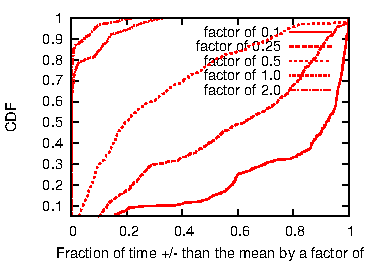
\includegraphics[width=0.4\textwidth] {figures/spatial-similarity.pdf}
\tightcaption{Spatial similarity of quality (average bitrate) among the sample of [Site, Initial CDN, Initial Bitrate, ASN, Site, ConnectionType, Object]. Each point represents a group of quality samples}
\label{fig:spatial-similarity}
\end{figure}

\myparasum{Spatial similarity} Spatial similarity is between the quality samples collected at the same time interval from sessions that share certain attribute values. \jc{Figure: x-Fraction of time less/greater than mean by various factor, y: CDF} Figure~\ref{fig:spatial-similarity} quantifies the similarity of average bitrate in quality samples that share the same tuple of Site, Initial CDN, Initial Bitrate, ASN, Site, ConnectionType, Object. It shows that there is a large fraction (more than 50\%) of quality sample groups that have less than 20\% of quality sample less or greater than the mean of this group with a factor of 0.5.

\begin{figure}[h!]
\centering
 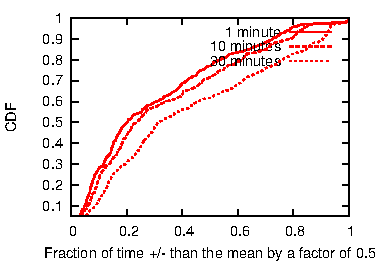
\includegraphics[width=0.4\textwidth] {figures/temporal-similarity.pdf}
\tightcaption{Quantifying impact of temporal distance on quality similarity. Figure shows likelihood of being more than a factor of 0.5 away from mean quality for all [Site, Initial CDN, Initial Bitrate, ASN, Site, ConnectionType, Object] groups with increasing (from left to right) time scales.}
\label{fig:temporal-similarity}
\end{figure}

\myparasum{Temporal similarity} Temporal similarity is between the average quality collected in different time interval of the same group of sessions that share certain attribute values. In Figure~\ref{fig:temporal-similarity}, we compare the similarity between quality samples with certain distance in time, and quantify the impact of temporal distance on quality similarity. Each point represents a group with the fraction of quality samples that is less or greater than the mean of the quality samples that have the same values on all seven attributes $t$ minutes ago ($t=1,10,30$). It shows that temporal distance does impact the quality similarity. 

\comment{
\myparasum{Summary of key observations} \jc{mostly based on my previous experience. subject to change after formal results are generated.}
\begin{packedenumerate}
	\item Both similarity of quality samples show that it is feasible to predict the quality of a new session and its decision by looking at quality samples that are spatially and temporally close to it.
	\item Spatial similarity varies across different attributes.  Using more attributes can improve things.
	\item Different quality metrics have different level of similarity, especially, buffering ratio has the largest similarity.
\end{packedenumerate}
}
}

\tightsubsection{Predicting from finite data}
Although the figures show that in many cases, quality is similar among quality samples that share the same attribute values and same temporal interval, there are still a lot of quality sample groups that have high dispersion as shown in the figure making it challenging for quality prediction. 
In this part, we enumerate the potential reasons that causes the dispersion we observe. To give an intuition, in case of small number of similar sessions, the mean quality outcome of a small sample of similar sessions (for example, $10$ such sessions) is subject to considerable random noise.  If we use that number for prediction, the prediction will be subject to the same noise and consequently to high average error.  As the number of attributes grows, quality grows more predictable (as we have seen) but the number of perfectly-matched sessions may drop exponentially.

Of course, prediction in the presence of limited information is the domain of statistics, and there are many potential solutions to this problem.  Any solution will deal with, and potentially trade off, four sources of prediction error:

\begin{packedenumerate}
  \item \emph{Estimation error:} In the statistical literature, prediction error due to limited data is often called {\it estimation error}.  Other things being equal, more data produce more accurate prediction. For example, Figure~\ref{fig:group-size-impact}-(a) presents the prediction error of using a group as a function of its (i.e., number of samples). To show  In fact, estimation error is a serious practical problem for video quality prediction.  Using all available attributes, many sessions have very few matches, as we would expect given the exponential explosion in combinations of attribute values.  

\begin{figure}[h!]
\centering
\subfigure[Prediction error vs. group size (w.r.t average bitrate)]
{
        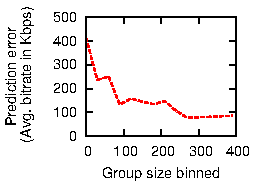
\includegraphics[width=110pt]{figures/count-err.pdf}
}
\subfigure[Distribution of group size]
{
        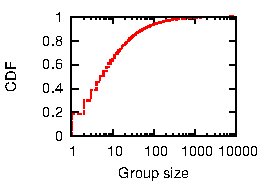
\includegraphics[width=110pt]{figures/count-cdf.pdf}
}
\tightcaption{Impact of group size (i.e., number of samples in a group). They show that more samples give more accuracy, and most of groups do not have sufficient samples for accurate prediction.}
\label{fig:group-size-impact}
\end{figure}

  \item \emph{Bias} due to missing or unused information: When grouping quality samples according to attributes we observe, we of course may not observe attributes that are important for prediction.  Say we do not observe (or use) important attribute X.  Then, even if we have infinitely many sessions that match the current session on all observed attributes, the average outcome for all of those sessions may be different from the average outcome for the subset of sessions that match the current session on attribute X.  This is a form of bias.  Predictability, as we have defined it, simply means low bias.  Importantly, it is not alleviated by gathering more session data; as we have seen, it may be alleviated by gathering more attributes about each session.
  \item \emph{Unavailability of recent data:} In a practical system, there are delays in measuring, sending and processing quality samples, so they are not available instantly.  If conditions change rapidly, there may be no quality samples sufficiently close to the session under prediction.  This is an extreme example of estimation error.  In this case it may be necessary to model the evolution of the video ecosystem over time in order to extrapolate to the current time. Figure~\ref{quality-variability} shows per-minute quality variability. It shows that even with sufficient data, the mean value of a group of quality samples could vary significantly.

\begin{figure}[h!]
\centering
 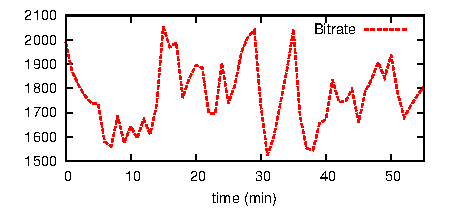
\includegraphics[width=0.4\textwidth] {figures/quality-time.pdf}
\tightcaption{Temporal variability of quality. The figure shows the mean value of average bitrate of a fixed group of same [Site, Initial CDN, Initial Bitrate, ConnectionType, ASN, Object], which has 100 quality samples in every minute in the figure.}
\label{fig:quality-variability}
\end{figure}

  \item \emph{Noise:} Even if we observed all conceivable attributes of a session and had infinitely many examples of exactly quality samples, outcomes may be affected by inputs that are practically random.  For example, performance may be affected by randomized algorithms in the networking layer.  This implies that some degree of prediction error is inevitable.
\end{packedenumerate}

More formally, we can derive this as follows (see \cite{domingos2000unified} for a less specialized discussion of the decomposition of prediction error).  Let $D$ be a set of quality samples from which a prediction algorithm learns its predictions.  Let $p_i$ be predicted quality for session $i$ and $q_i$ be its actual quality.  We further assume that $q_i$ is fixed except for an independent additive noise component, i.e. $q_i = \hat{q}_i + \epsilon_i$, where $\hat{q}_i$ is nonrandom and $\epsilon_i$ is a random variable with mean $0$, independent of $p_i$.  Then the mean squared prediction error, with respect to randomness in the observed data $D$ used to compute $p_i$, is:
\begin{align}
  \label{eqn:biasvariance}
  \E_D[(p_i - q_i)^2] &= \Var_D[p_i - q_i] + (\E_D[p_i - q_i])^2
\end{align}
\begin{align*}
  \label{eqn:biasvariancelong}
  &= \Var_D[p_i - \hat{q}_i - \epsilon_i] + (\E_D[p_i - \hat{q}_i - \epsilon_i])^2 \\
  &= \Var_D[p_i - \hat{q}_i] + \Var_D[\epsilon_i] + (\E_D[p_i - \hat{q}_i - \epsilon_i])^2\\
  &= \Var_D[p_i] + \Var_D[\epsilon_i] + (\E_D[p_i - \hat{q}_i - \epsilon_i])^2\\
  &= \Var_D[p_i] + \Var_D[\epsilon_i] + (\E_D[p_i - \hat{q}_i] - \E_D[\epsilon_i])^2\\
  &= \Var_D[p_i] + \Var_D[\epsilon_i] + (\E_D[p_i] - \hat{q})^2
\end{align*}

The first term in equation \eqref{eqn:biasvariancelong} is estimation error -- the variability in predictions across possible sets of observed data.  It will increase as the number of sessions similar to session $i$ in $D$ decreases; as a special case it may be very large if only a few quality samples in $D$ are temporally close to session $i$.  The second term is noise.  The third term is the squared bias of the predictor, which does not generally decrease with the size of $D$.  The prediction algorithm's average prediction error is simply the average over all sessions $i$ of the sum of these three terms.

\tightsubsection{Aggregation}
A simple strategy to reduce estimation error is {\it aggregation}~\cite{any citation?}.  By aggregation we mean putting quality samples into coarser groups that match on only a subset of observed attributes.  Aggregation increases the number of samples in each group but reduces the number of attributes, thus reducing estimation error at the cost of increased bias. 
Intuitively, when estimation error is small (say, when a fine-grained group contains many sessions) we want to eliminate bias by using a fine-grained group.  When estimation error is large, we want to aggregate more.  Figure \fillme demonstrates this for \fillme\jc{nice to have a figure to confirm such tradeoff does happen in our dataset.}.  This indicates that a prediction algorithm that uses aggregation should pay attention to its error rate to determine the right degree of aggregation.
Thus it makes sense to look for an optimal attribute combination, optimal AC (i.e., optimal degree of aggregation) \jc{remember to define AC earlier}. 

The optimal AC is defined with the assumption that all sessions under prediction sharing the same values on all attributes (i.e., identical under the finest AC) are given the same prediction and the optimal AC is the degree of aggregation that gives the prediction value which minimizes the standard deviation (i.e., the prediction values closest to the mean of the actual quality of these sessions). For instance, Figure~\ref{fig-optimal-AC.pdf} gives the hierarchy before time $t$ which consists of different degrees of aggregation (i.e., ACs) of the same finest group ``$ASN-1,CDN-1,Site-1$'' with all attributes specified. Now, givem a set of sessions at time $t$ and the mean of their real quality is 0.2, the optimal AC (colored in red) is the one with the closest prediction to 0.2, i.e., (ASN,CDN). The optimal AC is effectively an oracle approach since we assume the knowledge of actual quality. Except that, the optimal AC is operational as it makes prediction purely based on attribute. We will compare our practical algorithm with this oracle in \Section~\ref{sec:prediction}

By studying the distribution of optimal AC, we find that the optimal AC (the aggregation that gives minimal prediction error) is in many cases neither the finest nor the coarsest one and is highly dynamic. 



\begin{figure}[h!]
\centering
 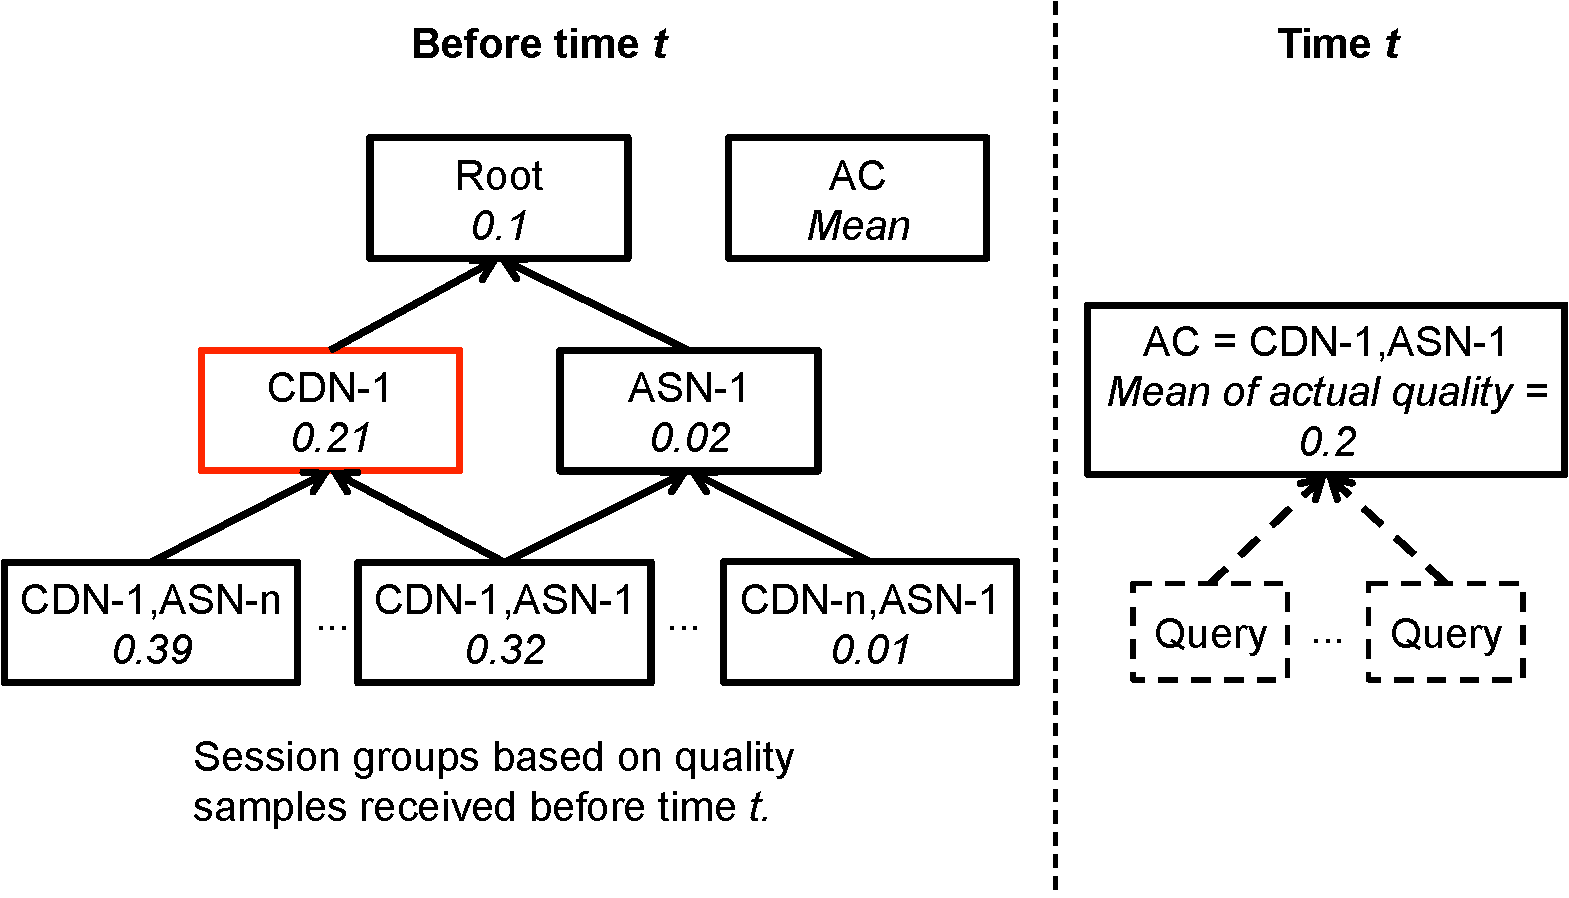
\includegraphics[width=0.5\textwidth] {figures/fig-optimal-AC.pdf}
\tightcaption{Example of how optimal AC is identified. The optimal AC is colored in red. Assuming the considered attributes are fixed, the optimal AC assumes that all sessions that belong to the same finest group should be given the same prediction, and the optimal AC is the one that gives the closest prediction among those that contain this finest group.}
\label{fig:example-optimal-ac}
\end{figure}

Figure~\ref{fig:optimal-ac-dynamics}-(a) gives coverage of optimal ACs (for each AC, the fraction of sessions of which this AC is the optimal AC), and it shows that the finest group only has coverage about 20\% and no coarsest grain AC (single attribute) is among the top 5. This implies that the optimal AC often occurs between the finest and coarsest grainular.
Figure~\ref{fig:optimal-ac-dynamics}-(b) gives prevalence of pair of (session under prediction, optimal AC) (the fraction of time that the finest group has this optimal AC), and it shows that 70\% pairs of (session under prediction, optimal AC) only last for less than 20\% of time. This implies that no single or a small set of optimal AC that can cover most sessions and used statically.
Figure~\ref{fig:optimal-ac-dynamics}-(c) gives persistence of pair of (session under prediction, optimal AC) (the longest continuous duration where a finest group has the same optimal AC) and it shows that there is at most 40\% of pair of (session under prediction, optimal AC) last more than 10 minutes. This implies that even a reactive strategy will miss many optimal AC.

\begin{figure}[h!]
\centering
\subfigure[Distribution of coverage of top five optimal ACs (w.r.t averge bitrate).]
{
        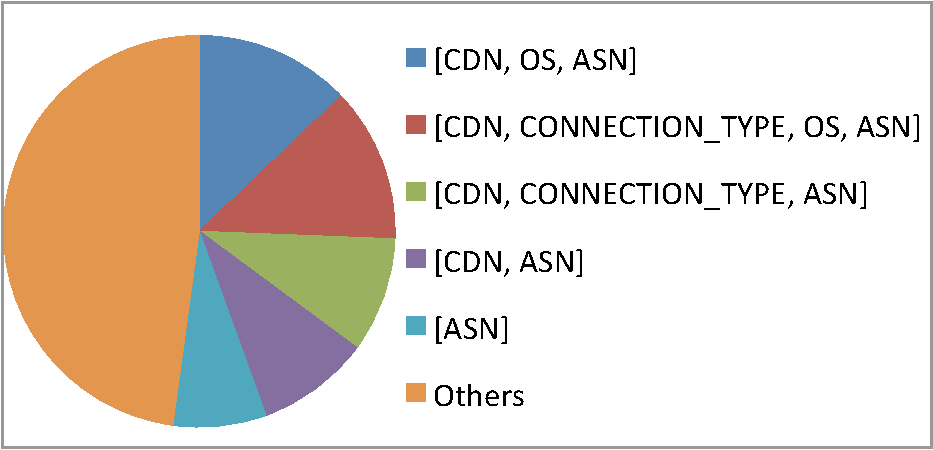
\includegraphics[width=0.4\textwidth]{figures/optimal_AC_distribution.pdf}
}
\subfigure[Prevalence of pair of (session under prediction, optimal AC).]
{
        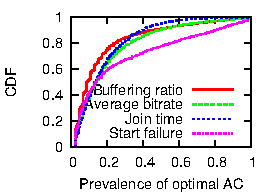
\includegraphics[width=0.3\textwidth]{figures/optimal-prevalence.pdf}
}
\subfigure[Persistence of pair of (session under prediction, optimal AC).]
{
        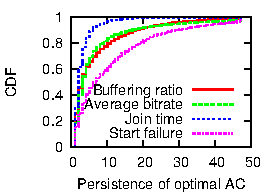
\includegraphics[width=0.3\textwidth]{figures/optimal-persistence.pdf}
}
\tightcaption{Dynamics of the optimal AC. (a) gives coverage of optimal ACs (for each AC, the fraction of sessions of which this AC is the optimal AC).
(b) gives prevalence of pair of (session under prediction, optimal AC) (the fraction of time that the finest group has this optimal AC).
(c) gives persistence of pair of (session under prediction, optimal AC) (i.e., the longest continuous duration where a finest group has the same optimal AC).}
\label{fig:optimal-ac-dynamics}
\end{figure}

